$for(header-includes)$
  $header-includes$
$endfor$

$if(loa)$
\makeglossaries
\newacronym{dnn}{DNN}{Deep Neural Network}

\newacronym{ar}{AR}{Augmented Reality}

\newacronym[longplural={Application Programming Interfaces}]{api}{API}{Application Programming Interface}

\newacronym{whnf}{WHNF}{weak head normal form}

\newacronym[longplural={Generalized algebraic datatypes},shortplural={GADTs}]{gadt}{GADT}{Generalized algebraic datatype}

\newacronym[longplural={Garbage Collection},shortplural={GC}]{gc}{GC}{Garbage Collector}

\newacronym{ghc}{GHC}{Glascow Haskell Compiler}

\newacronym{ghci}{GHCi}{GHC Interpreter}

\newacronym{rts}{RTS}{Runtime System}

\newacronym{stm}{STM}{Software Transactional Memory}

\newacronym{os}{OS}{Operating System}

\newacronym{ffi}{FFI}{Foreign Function Interface}

\newacronym{lhs}{LHS}{Left-hand side}

\newacronym{rhs}{RHS}{Right-hand side}

$endif$

%%%%%%%%%%%%%%%%%%%%%%%%%%%%%%%%%%%%%%%%%%%%%%%%%%%%%%%%%%%%% Document beginning.
\begin{document}

$if(title)$
% Include custom titlepage
\prefrontmatter
\thispagestyle{empty}             % No page numbers
\calccentering{\unitlength}
\begin{adjustwidth*}{\unitlength}{-\unitlength}
    \begin{adjustwidth}{-0.5cm}{-0.5cm}
        \sffamily
        \begin{flushright}
            \thesistypeabbr{} Thesis\\*[0cm]
            \thesistype{}\\        \end{flushright}
        \vspace*{\fill}
        \noindent
        
\includegraphics[width=0.75\textwidth]{Graphic/Titlepage/DTU Fotonik}\\*[0.5cm]
        \HUGE \thesistitle{}\\*[0.2cm]
        \Large \thesissubtitle{}\\*[1.2cm]
        \parbox[b]{0.7\linewidth}{%
            \Large
            \thesisauthor{}\\*[1.2cm]
            \Large
            \thesislocation{} \the\year
        }
        \hfill\begin{tabular}{cc}
            
\includegraphics[scale=0.7]{Graphic/Titlepage/KAIST Logo} \hspace{0.1cm} & 
\includegraphics[scale=1.2]{Graphic/Titlepage/DTU Logo}
        \end{tabular}
    \end{adjustwidth}
\end{adjustwidth*}
\normalfont
\normalsize

\cleartoevenpage

$endif$

$if(thesis.colophon)$
\thispagestyle{empty} % No page numbers
\frieze
\vspace*{\fill}
\noindent
\sffamily
\scriptsize
\textbf{\thesisinstitute{}}\\
\textbf{\thesisinstitutelongname{}}\\
\textbf{\thesisuniversity{}}\\
\\
\thesisaddress{}\\
\normalsize
\normalfont
\vspace*{1.5cm}

\cleartooddpage
$endif$

\frontmatter
% \pagenumbering{roman}
% \setcounter{page}{1}

$if(abstract)$
\chapter*{Abstract}
\addcontentsline{toc}{chapter}{Abstract}
\setcounter{chapter}{0}
$abstract$
\clearforchapter
$endif$

$if(preface)$
\chapter*{Preface}
\addcontentsline{toc}{chapter}{Preface}
\setcounter{chapter}{0}
$preface$
\clearforchapter
$endif$

% Items to include before the document.
$for(include-before)$
$include-before$

$endfor$

% Table of contents.
$if(toc)$
{
$if(colorlinks)$
  \hypersetup{linkcolor=$if(toccolor)$$toccolor$$else$black$endif$}
$endif$
\setcounter{tocdepth}{$toc-depth$}
\tableofcontents
}
\clearforchapter
$endif$

% List of tables.
$if(lot)$
\listoftables
\clearforchapter
$endif$

% List of figures.
$if(lof)$
\listoffigures
\clearforchapter
$endif$

$if(loa)$
%\printglossary[type=\acronymtype]
%\clearforchapter
$endif$

$if(lol)$
\listoflistings
\markboth{List of Listings}{}
\addcontentsline{toc}{chapter}{List of Listings}
\clearforchapter
$endif$

% The actual content of the document.
\mainmatter
$body$

\appendix
\chapter{Comparison of Results}\label{app:comparison_of_results}

% 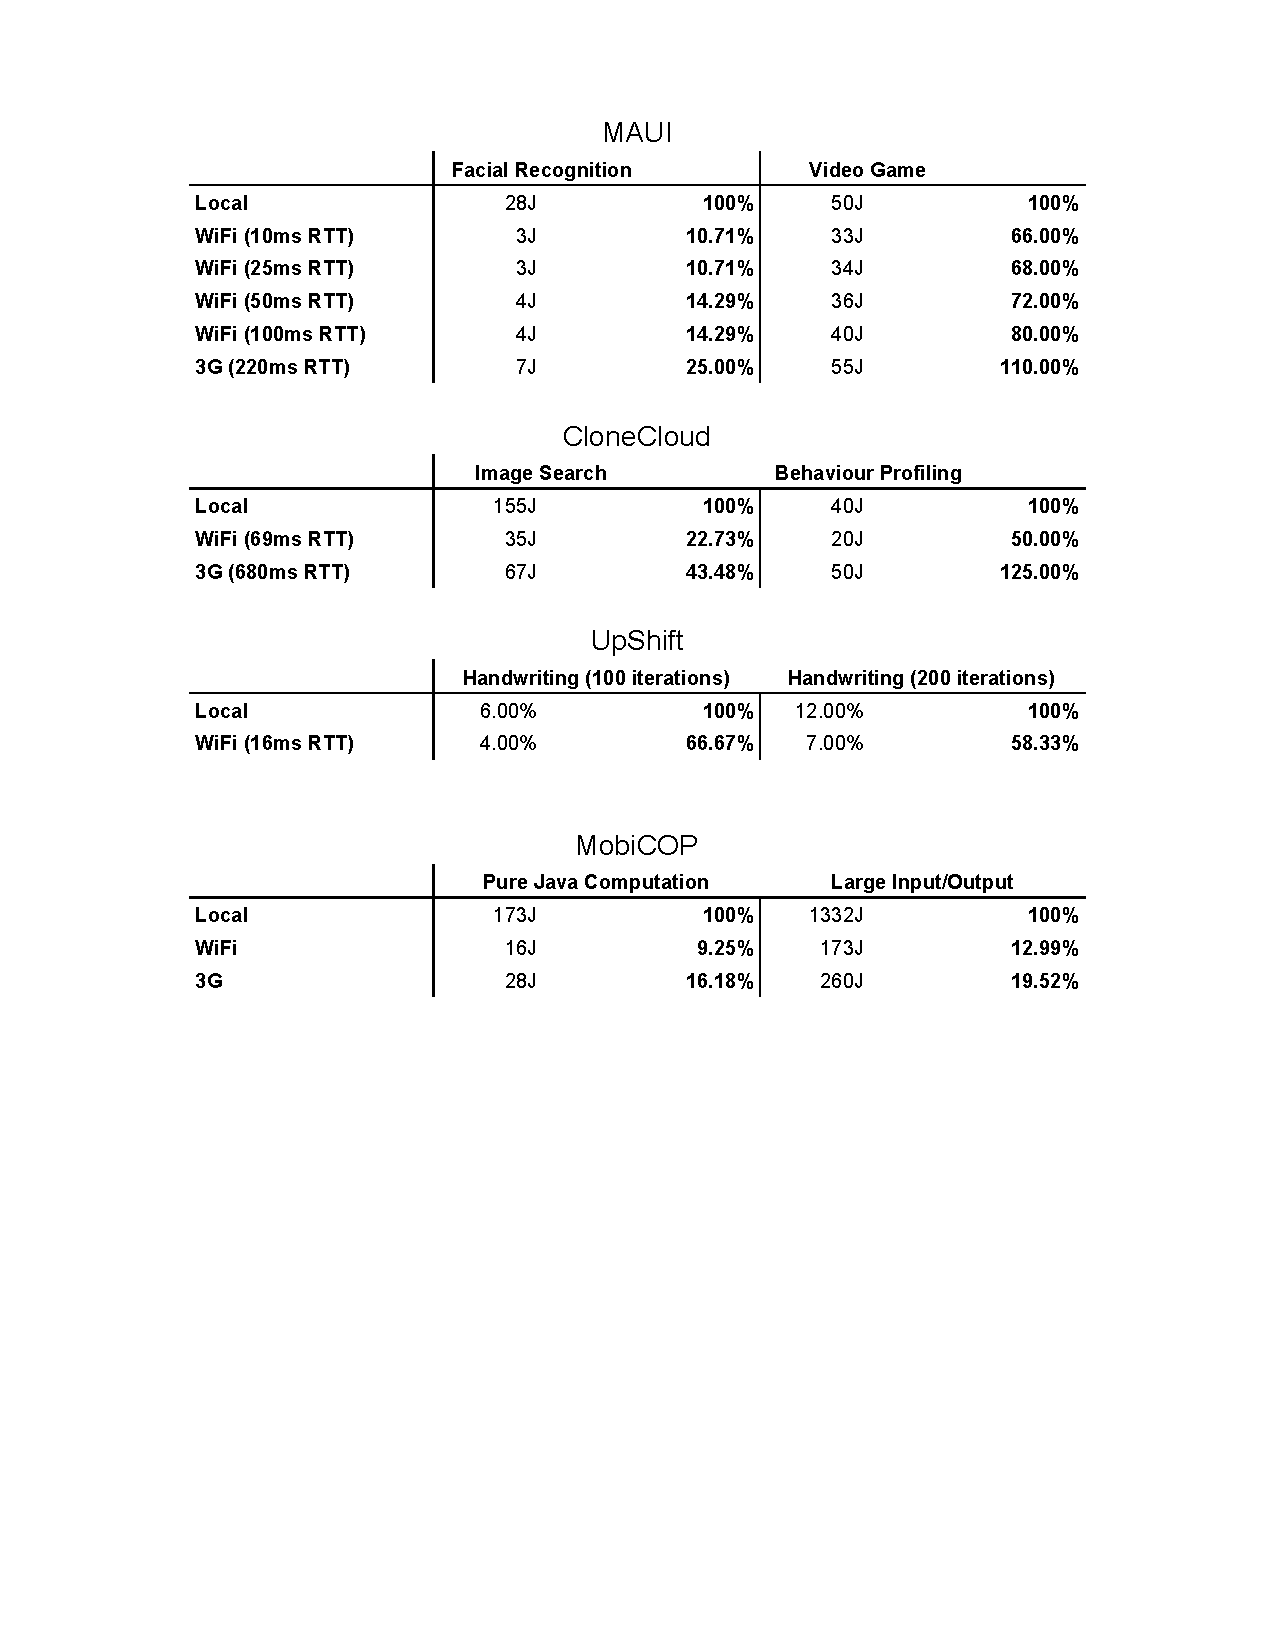
\includepdf[pages={1}]{Appendix/Comparison of Results.pdf}
\begin{figure}[h]
  \centering
  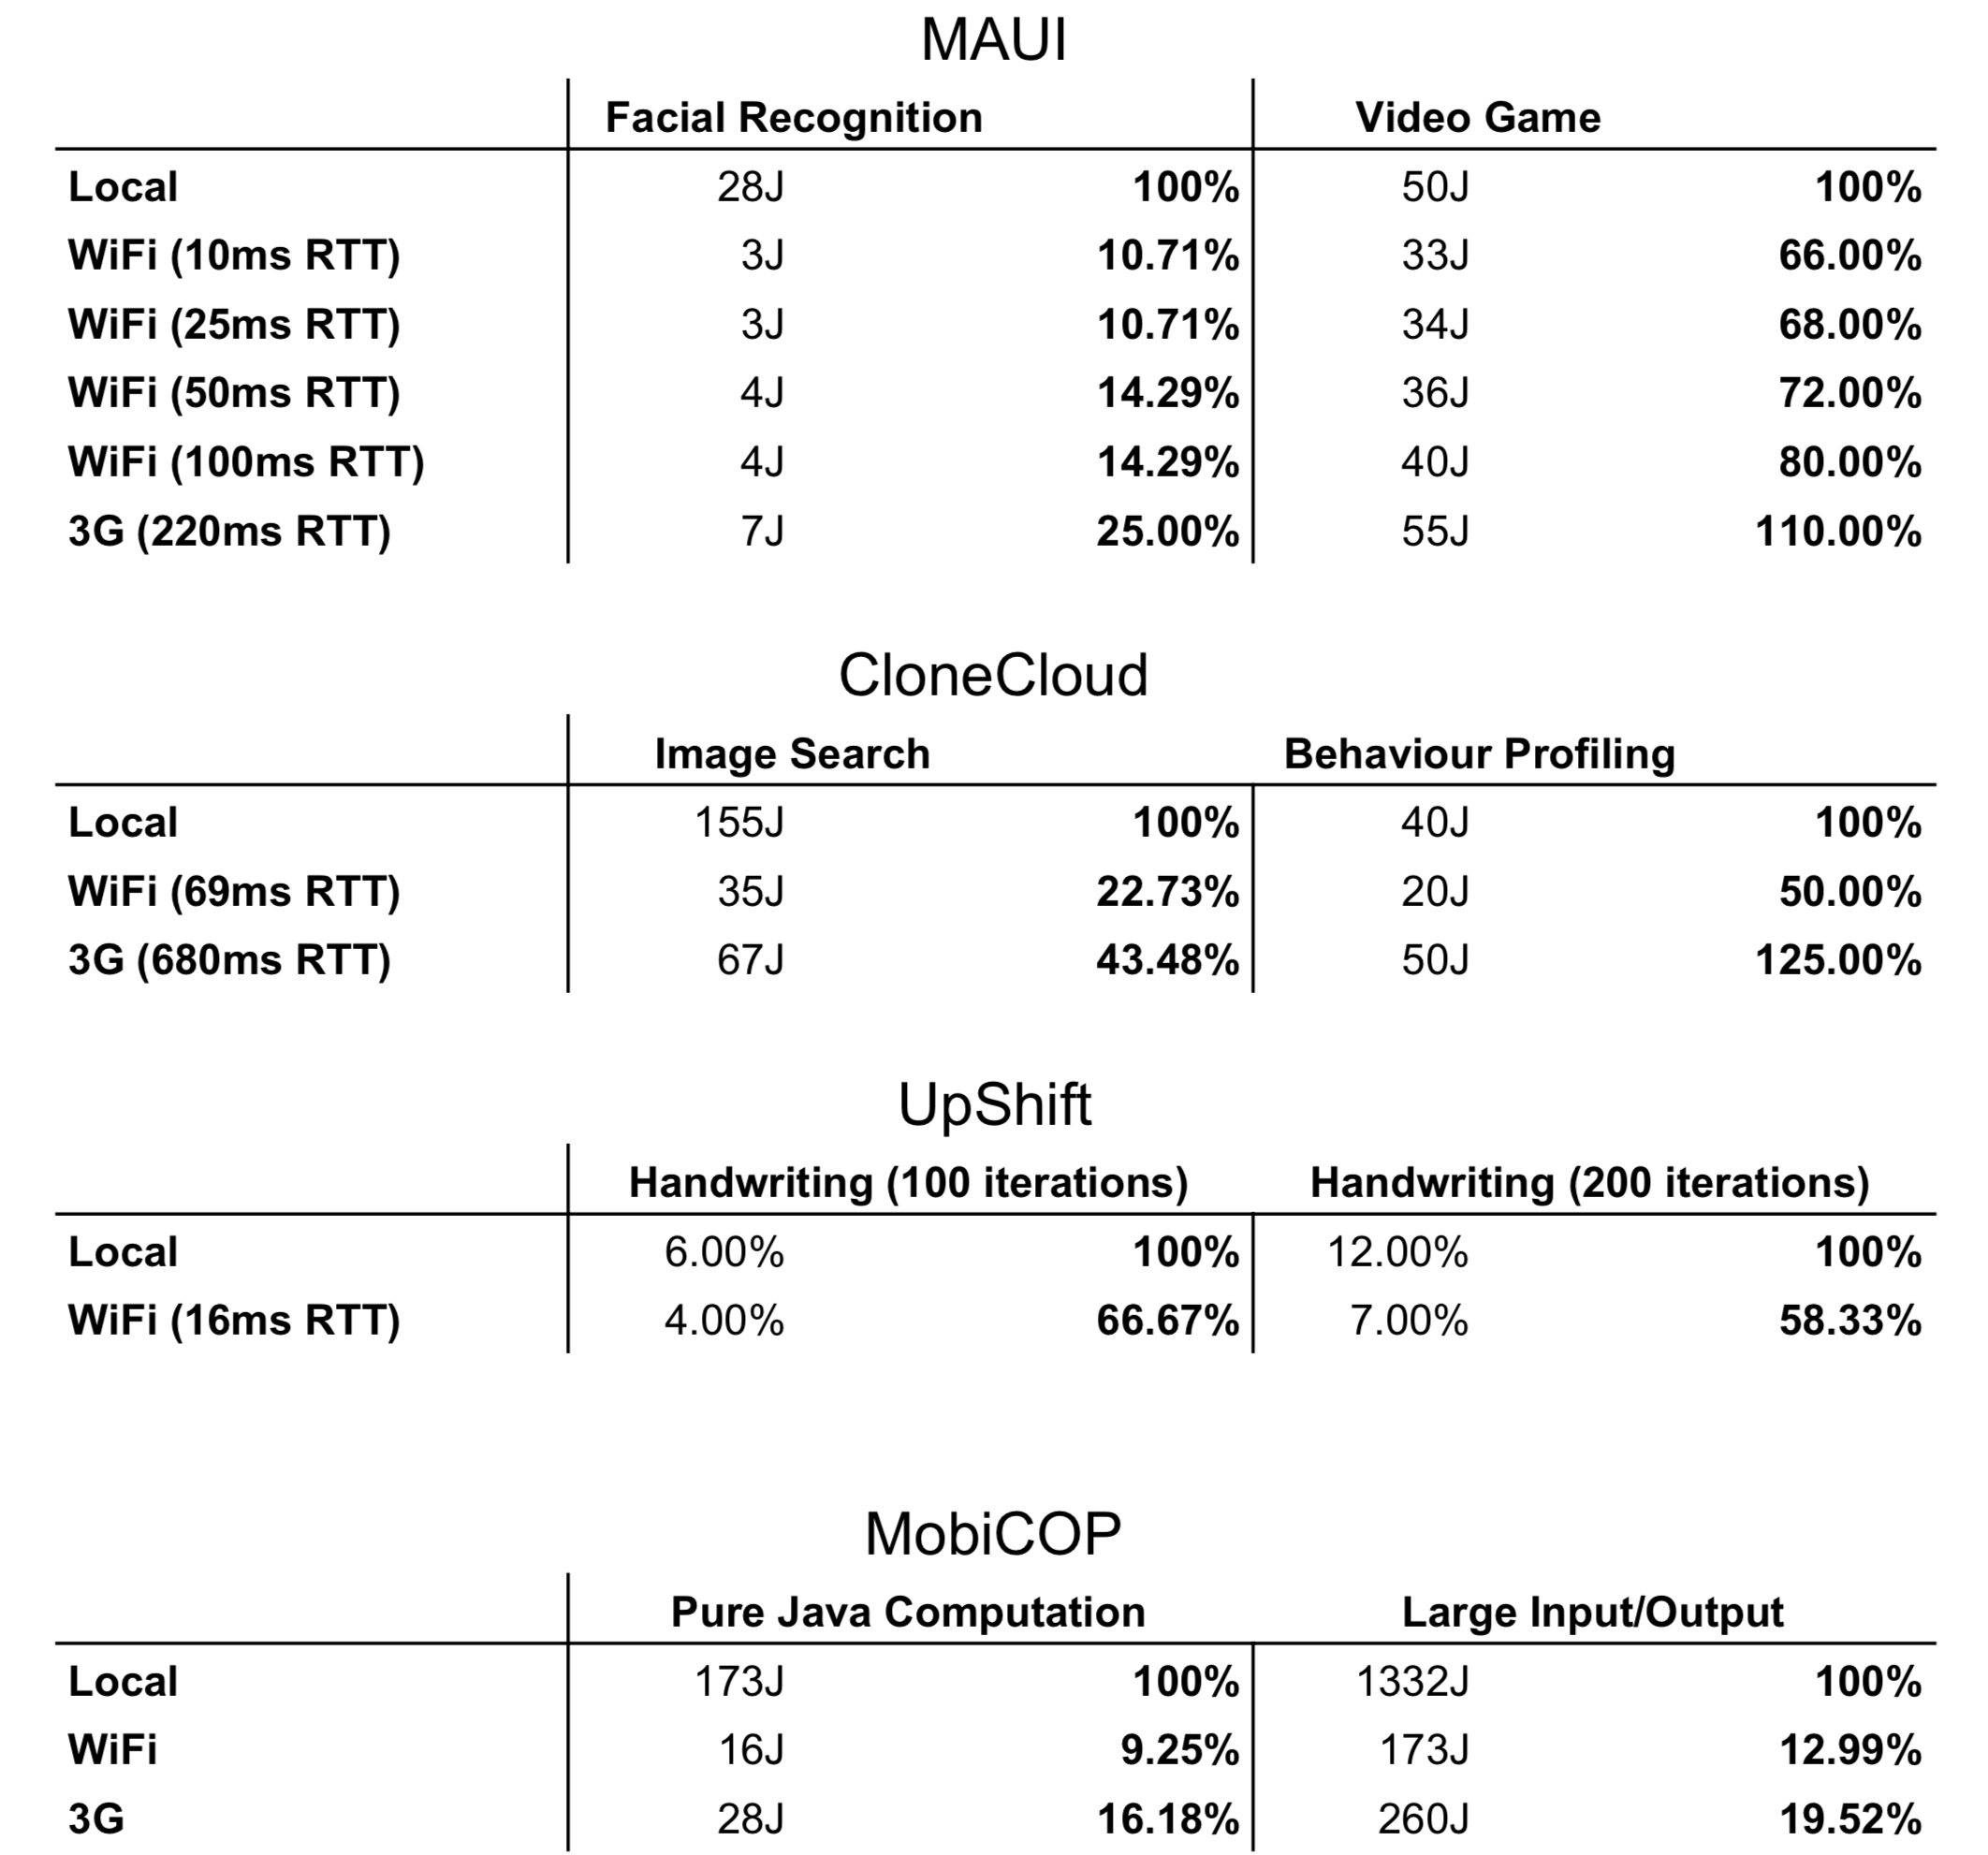
\includegraphics[page=1,width=1\textwidth]{Appendix/Comparison of Results.png}
\end{figure}

% Bibliography.
\backmatter
$if(natbib)$
  $if(bibliography)$
  $if(biblio-title)$
  $if(book-class)$
  \renewcommand\bibname{$biblio-title$}
  $else$
  \renewcommand\refname{$biblio-title$}
  $endif$
  $endif$
  \bibliography{$for(bibliography)$$bibliography$$sep$,$endfor$}

  $endif$
$endif$

% Printing the Bibliography if biblatex.
$if(biblatex)$
\printbibliography$if(biblio-title)$[heading=bibintoc,title={$biblio-title$}]$endif$

$endif$

% Items to include after the document.
$for(include-after)$
$include-after$

$endfor$

\end{document}
